\documentclass[11pt, twocolumn]{article}  % for review and submission
%\documentclass[aps,preprint,showpacs,superscriptaddress,groupedaddress]{revtex4}  % for double-spaced preprint
\usepackage{graphicx}  % needed for figures
\usepackage{dcolumn}   % needed for some tables
\usepackage{bm}        % for math
\usepackage{amssymb}   % for math
\usepackage{hyperref}  %to use \autoref to reference objects
\usepackage[export]{adjustbox} %alignment of figures

%\linespread{1.8} %double-spacing

\usepackage[hmarginratio=1:1,top=15mm, bottom=15mm, left=15mm, right=15mm,columnsep=20pt]{geometry} % Document margins
%\usepackage{anysize}
%\marginsize{20mm}{20mm}{15mm}{15mm}
%\marginsize{left}{right}{top}{bottom}
%\usepackage[left = 15mm, top = 15mm]{geometry} %margins

\providecommand{\e}[1]{\ensuremath{\times 10^{#1}}} %for scientific notation
\providecommand{\squiggle}{\raise.17ex\hbox{$\scriptstyle\sim$}} %for tilde character
\providecommand{\neus}{$n_{e~upstream}$} % upstream electron density shortcut


%\usepackage[left = 15mm, top = 15mm]{geometry} %margins
\usepackage{amssymb} % Allows use of \therefore command to get the three dots in a triangle symbol

%Figures
\usepackage{graphicx}
%syntax:
%\includegraphics[scale=1.0]{filepath.extension}

%bibliog
\usepackage[UKenglish]{babel}
\usepackage{url}
\usepackage[backend=bibtex, style=numeric-comp, sorting=none, doi=false,isbn=false,url=false]{biblatex}
\bibliography{BIBfiles/initial}
% bun citep amirite!!!
\newcommand{\citep}[1]{\cite{#1}}
%stop paper titles being printed in bibliography
\AtEveryBibitem{\clearfield{title}}
%stop "In:" being printed before journal name
\renewbibmacro{in:}{}
%small bibliography font size
\renewcommand*{\bibfont}{\small}

% Appendix
\usepackage[toc,page]{appendix}
%euro symbol (\EUR i think)
\usepackage{eurosym}

% Document
\begin{document}

\title{Divertor detachment stability and dynamics}
\author{Joe Allen, JOA509}
%\date{\today}

\twocolumn[
\begin{@twocolumnfalse}
    \maketitle
    \begin{abstract}
\noindent Do I need an abstract? Well, if I do then it will go here, spread over both columns. 
	\end{abstract}
\end{@twocolumnfalse}
]

%\tableofcontents

\section{Introduction}\label{sec:Intro}

\section{Background}\label{sec:Bg}
Brief overview of the importance of detachment for ITER and future tokamaks.
- Current material limit
- Divertor geometries (conventional, super-X, snowflake)
- 


\section{Experimental Design}\label{sec:Expt}
SOL1D was installed on the remote server and some test simulations run to achieve a basic understanding of the set-up and outputs. The first aim was to ascertain an acceptable grid resolution to use, as a compromise is required concerning accuracy of results and time taken to run a simulation. SOL1D performs 1-dimensional simulations and the y-axis was chosen as the simulation axis. 




Following SOL1D simulations, 2D simulations followed, with the initial goal being to compare results to the 1D case.


\section{Results and Analysis}\label{sec:Results}
After a number of time-steps of SOL1D simulation it will usually settle down and get close to a steady-state solution. This can be seen in figure~\ref{fig:ne_var_ny=800} - the variable's, \neus, oscillations are damped to a very small amplitude as the simulation progresses and it approaches steady-state.

\begin{figure}
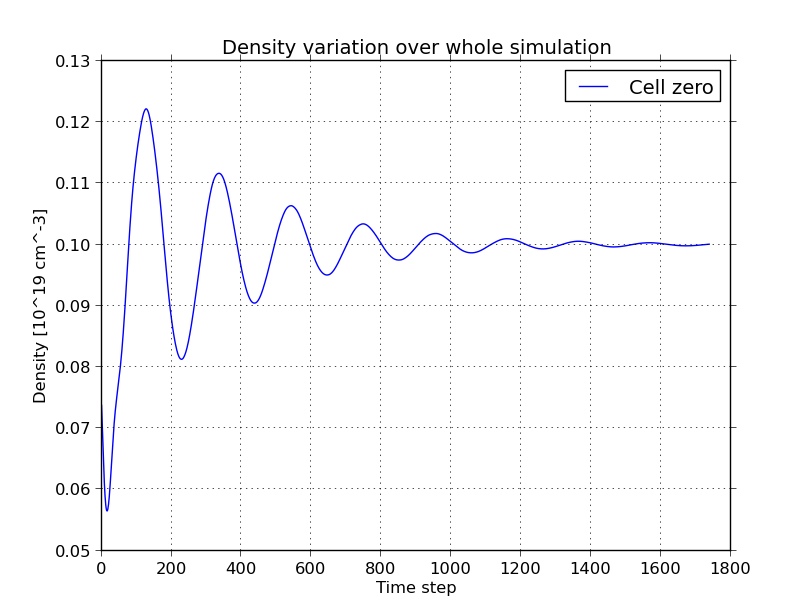
\includegraphics[scale=0.4]{Figures/sol1d/ne_var_ny=800.PNG}
\centering
\caption{The variation of \neus with simulation time step. \textbf{should maybe put the oscillations from other resolutions on the same figure to make it more interesting?}}\label{fig:ne_var_ny=800}
\end{figure}



See figure~\ref{fig:TT_IMPCOMBO} for a nice graph.

\begin{figure}
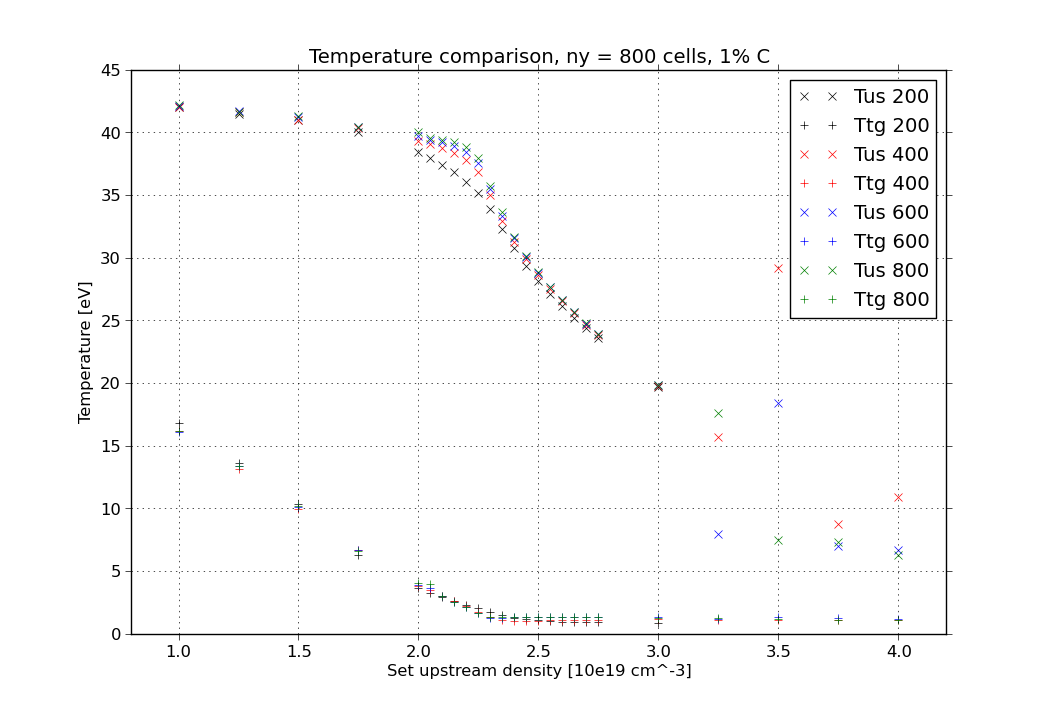
\includegraphics[scale=0.4]{Figures/sol1d/TT_IMPCOMBO.PNG}
\centering
\caption{Comparison of $T_{upstream}$ and $T_{target}$ at varying set $n_{e~upstream}$ for different y-axis resolutions in SOL1D}\label{fig:TT_IMPCOMBO}
\end{figure}

\section{Conclusion}\label{sec:Conclusion}




\printbibliography

\end{document}
